\documentclass[10pt, aspectratio=169]{beamer}

% Theme selection
\usetheme{Madrid}
\usecolortheme{seahorse}

% Packages
\usepackage{graphicx}
\usepackage{booktabs}
\usepackage{amsmath, amssymb}
\usepackage{xcolor}
\usepackage{colortbl}
\usepackage{caption}

% Custom Color Palette
\definecolor{primaryblue}{RGB}{13, 71, 161}
\definecolor{secondaryblue}{RGB}{25, 118, 210}
\definecolor{accentorange}{RGB}{230, 81, 0}
\definecolor{darkgreen}{RGB}{27, 94, 32}
\definecolor{lightbg}{RGB}{245, 247, 250}

\setbeamercolor{palette primary}{bg=primaryblue, fg=white}
\setbeamercolor{palette secondary}{bg=secondaryblue, fg=white}
\setbeamercolor{palette tertiary}{bg=primaryblue, fg=white}
\setbeamercolor{titlelike}{bg=primaryblue, fg=white}
\setbeamercolor{frametitle}{bg=primaryblue, fg=white}
\setbeamercolor{structure}{fg=primaryblue}

\setbeamertemplate{navigation symbols}{}
\setbeamertemplate{footline}[frame number]

% Title Information
\title[Next-Day 24-Hour Stock Status Prediction]{Next-Day 24-Hour Stock Status Prediction in Fresh Retail}
\subtitle{Architectural Evolution from LSTMs to Hourly Slot-Specific DLinear}
\author[Anurag, Samyak, Vibhor]{Anurag Thakur \quad Samyak \quad Vibhor Kumar}
\institute[BTP 2026]{Department of Information Technology\\Bachelor of Technology Project (BTP)}
\date{August 2026}

\begin{document}

% ==========================================
% SLIDE 1: TITLE SLIDE
% ==========================================
\begin{frame}
  \titlepage
\end{frame}

% ==========================================
% SLIDE 2: PROBLEM STATEMENT & OBJECTIVE METRICS
% ==========================================
\begin{frame}{Problem Statement \& Objective Metrics}
  \begin{columns}[T]
    \begin{column}{0.48\textwidth}
      \begin{block}{Operational Challenge in Fresh Retail}
        \begin{itemize}
          \item Perishable fresh items suffer from \textbf{rapid intra-day demand shocks} and supply replenishment lags.
          \item Unpredicted stockouts cause direct financial revenue loss, stock spoilage, and customer churn.
        \end{itemize}
      \end{block}
      
      \begin{block}{Predictive Target Formulation}
        \begin{itemize}
          \item Forecast a \textbf{24-dimensional binary hourly status vector}:
            $$\mathbf{Y} = [y_1, y_2, \dots, y_{24}]^T \in \{0, 1\}^{24}$$
          \item Covers active operational store hours (\textbf{6 AM to 10 PM}).
          \item $y_h = 1$ indicates SKU stockout during hour $h$.
        \end{itemize}
      \end{block}
    \end{column}
    
    \begin{column}{0.48\textwidth}
      \begin{exampleblock}{Key Objective Performance Metrics}
        \begin{itemize}
          \item \textbf{Hour-Level F1-Score} (Primary Metric): Evaluates precision vs. recall on positive stockout hours:
            $$F1 = \frac{2 \cdot P \cdot R}{P + R}$$
          \item \textbf{Stockout Recall}: Measures percentage of true operational stockout hours correctly detected ($R = \frac{TP}{TP + FN}$).
          \item \textbf{Exact 24-Hour Match Rate}: Proportion of days where all 24 hourly predictions match ground truth exactly.
          \item \textbf{Mean Absolute Error (MAE)}: Average absolute error in total daily stockout duration (in hours).
        \end{itemize}
      \end{exampleblock}
    \end{column}
  \end{columns}
\end{frame}

% ==========================================
% SLIDE 3: LITERATURE REVIEW & RELATED WORK
% ==========================================
\begin{frame}{Literature Review \& Related Work}
  \begin{block}{Taxonomy of Time-Series Forecasting Literature}
    \begin{itemize}
      \item \textbf{Recurrent Sequence Memory} (Hochreiter \& Schmidhuber, 1997):
        \textit{LSTM} maintains persistent cell state memory $C_t$ for temporal sequence continuity.
      \item \textbf{Limitations of Daily Aggregation} (Syntetos et al., 2016):
        Traditional models predict coarse 1-day scalar demand, obscuring intraday stockout timing.
      \item \textbf{Deep Time-Series Transformers} (Lim et al., 2021 [TFT]; Zeng et al., 2023 [PatchTST]):
        Self-attention mechanisms suffer from \textbf{overparameterization ($>280\text{k}$ params)} on short sequences.
      \item \textbf{Linear Series Decomposition} (Zeng et al., 2023 [DLinear]; Challu et al., 2023 [N-HiTS]):
        Moving-average trend decomposition provides parameter-efficient baselines ($<15\text{k}$ params).
      \item \textbf{Explainable AI in Retail} (Sundararajan et al., 2017 [IG]; Lundberg \& Lee, 2017 [SHAP]):
        Attribution methods reveal feature-level importance to guide neural architecture design.
    \end{itemize}
  \end{block}
\end{frame}

% ==========================================
% SLIDE 4: DATASET & SKU SELECTION STRATEGY
% ==========================================
\begin{frame}{Data Selection Strategy: FreshRetailNet-50K \& SKU Scoring}
  \begin{block}{Unit of Analysis}
    Time series defined at individual SKU-store grain: 
    $$\text{series\_id} = \text{city\_id} + \text{store\_id} + \text{product\_id}$$
  \end{block}

  \begin{columns}[T]
    \begin{column}{0.50\textwidth}
      \begin{block}{Why Statistically Filter SKUs?}
        \begin{itemize}
          \item Large fresh retail datasets contain thousands of dormant SKUs.
          \item We focus evaluation on \textbf{high-impact, stockout-prone SKUs} driving over 80\% of store revenue loss.
        \end{itemize}
      \end{block}
    \end{column}
    
    \begin{column}{0.46\textwidth}
      \begin{block}{SKU Statistical Ranking Formula}
        $$\begin{aligned}
          \text{Score} &= 0.40 \cdot \text{Sales} + 0.25 \cdot \text{StockoutHours} \\
          &+ 0.20 \cdot \text{StockoutDays} + 0.15 \cdot \text{SalesStd}
        \end{aligned}$$
      \end{block}
    \end{column}
  \end{columns}
  
  \vspace{4pt}
  \centering
  \small{\textbf{Selected Top 15 SKUs}: Represent high-turnover perishable items with high demand variance.}
\end{frame}

% ==========================================
% SLIDE 5: HOURLY VS DAILY FORECASTING PARADIGM
% ==========================================
\begin{frame}{Hourly vs. Daily Forecasting Paradigm}
  \begin{columns}[T]
    \begin{column}{0.48\textwidth}
      \begin{alertblock}{Traditional Daily Aggregation Paradigm}
        \begin{itemize}
          \item \textbf{Input}: $L=14$ days of historical daily metrics.
          \item \textbf{Output}: 1 scalar value (Total expected daily sales or binary stockout flag).
          \item \textbf{Loss of Information}: Store managers cannot determine \emph{when} replenishment must occur.
        \end{itemize}
      \end{alertblock}
    \end{column}
    
    \begin{column}{0.48\textwidth}
      \begin{exampleblock}{Our 24-Hour Hourly Binary Paradigm}
        \begin{itemize}
          \item \textbf{Input}: $L=14$ days of SKU-store daily feature vectors.
          \item \textbf{Output}: 24 binary probabilities $\hat{\mathbf{Y}} \in [0, 1]^{24}$.
          \item \textbf{Actionable Insight}: Identifies peak risk hours (e.g. 11 AM lunch rush \& 6 PM evening peak) for proactive restocking.
        \end{itemize}
      \end{exampleblock}
    \end{column}
  \end{columns}
\end{frame}

% ==========================================
% SLIDE 6: INITIAL BENCHMARK: LSTM VS TRANSFORMERS VS RNNS
% ==========================================
\begin{frame}{Model Family Comparison: Simple LSTMs Beat Heavy Transformers}
  \begin{columns}[T]
    \begin{column}{0.58\textwidth}
      \centering
      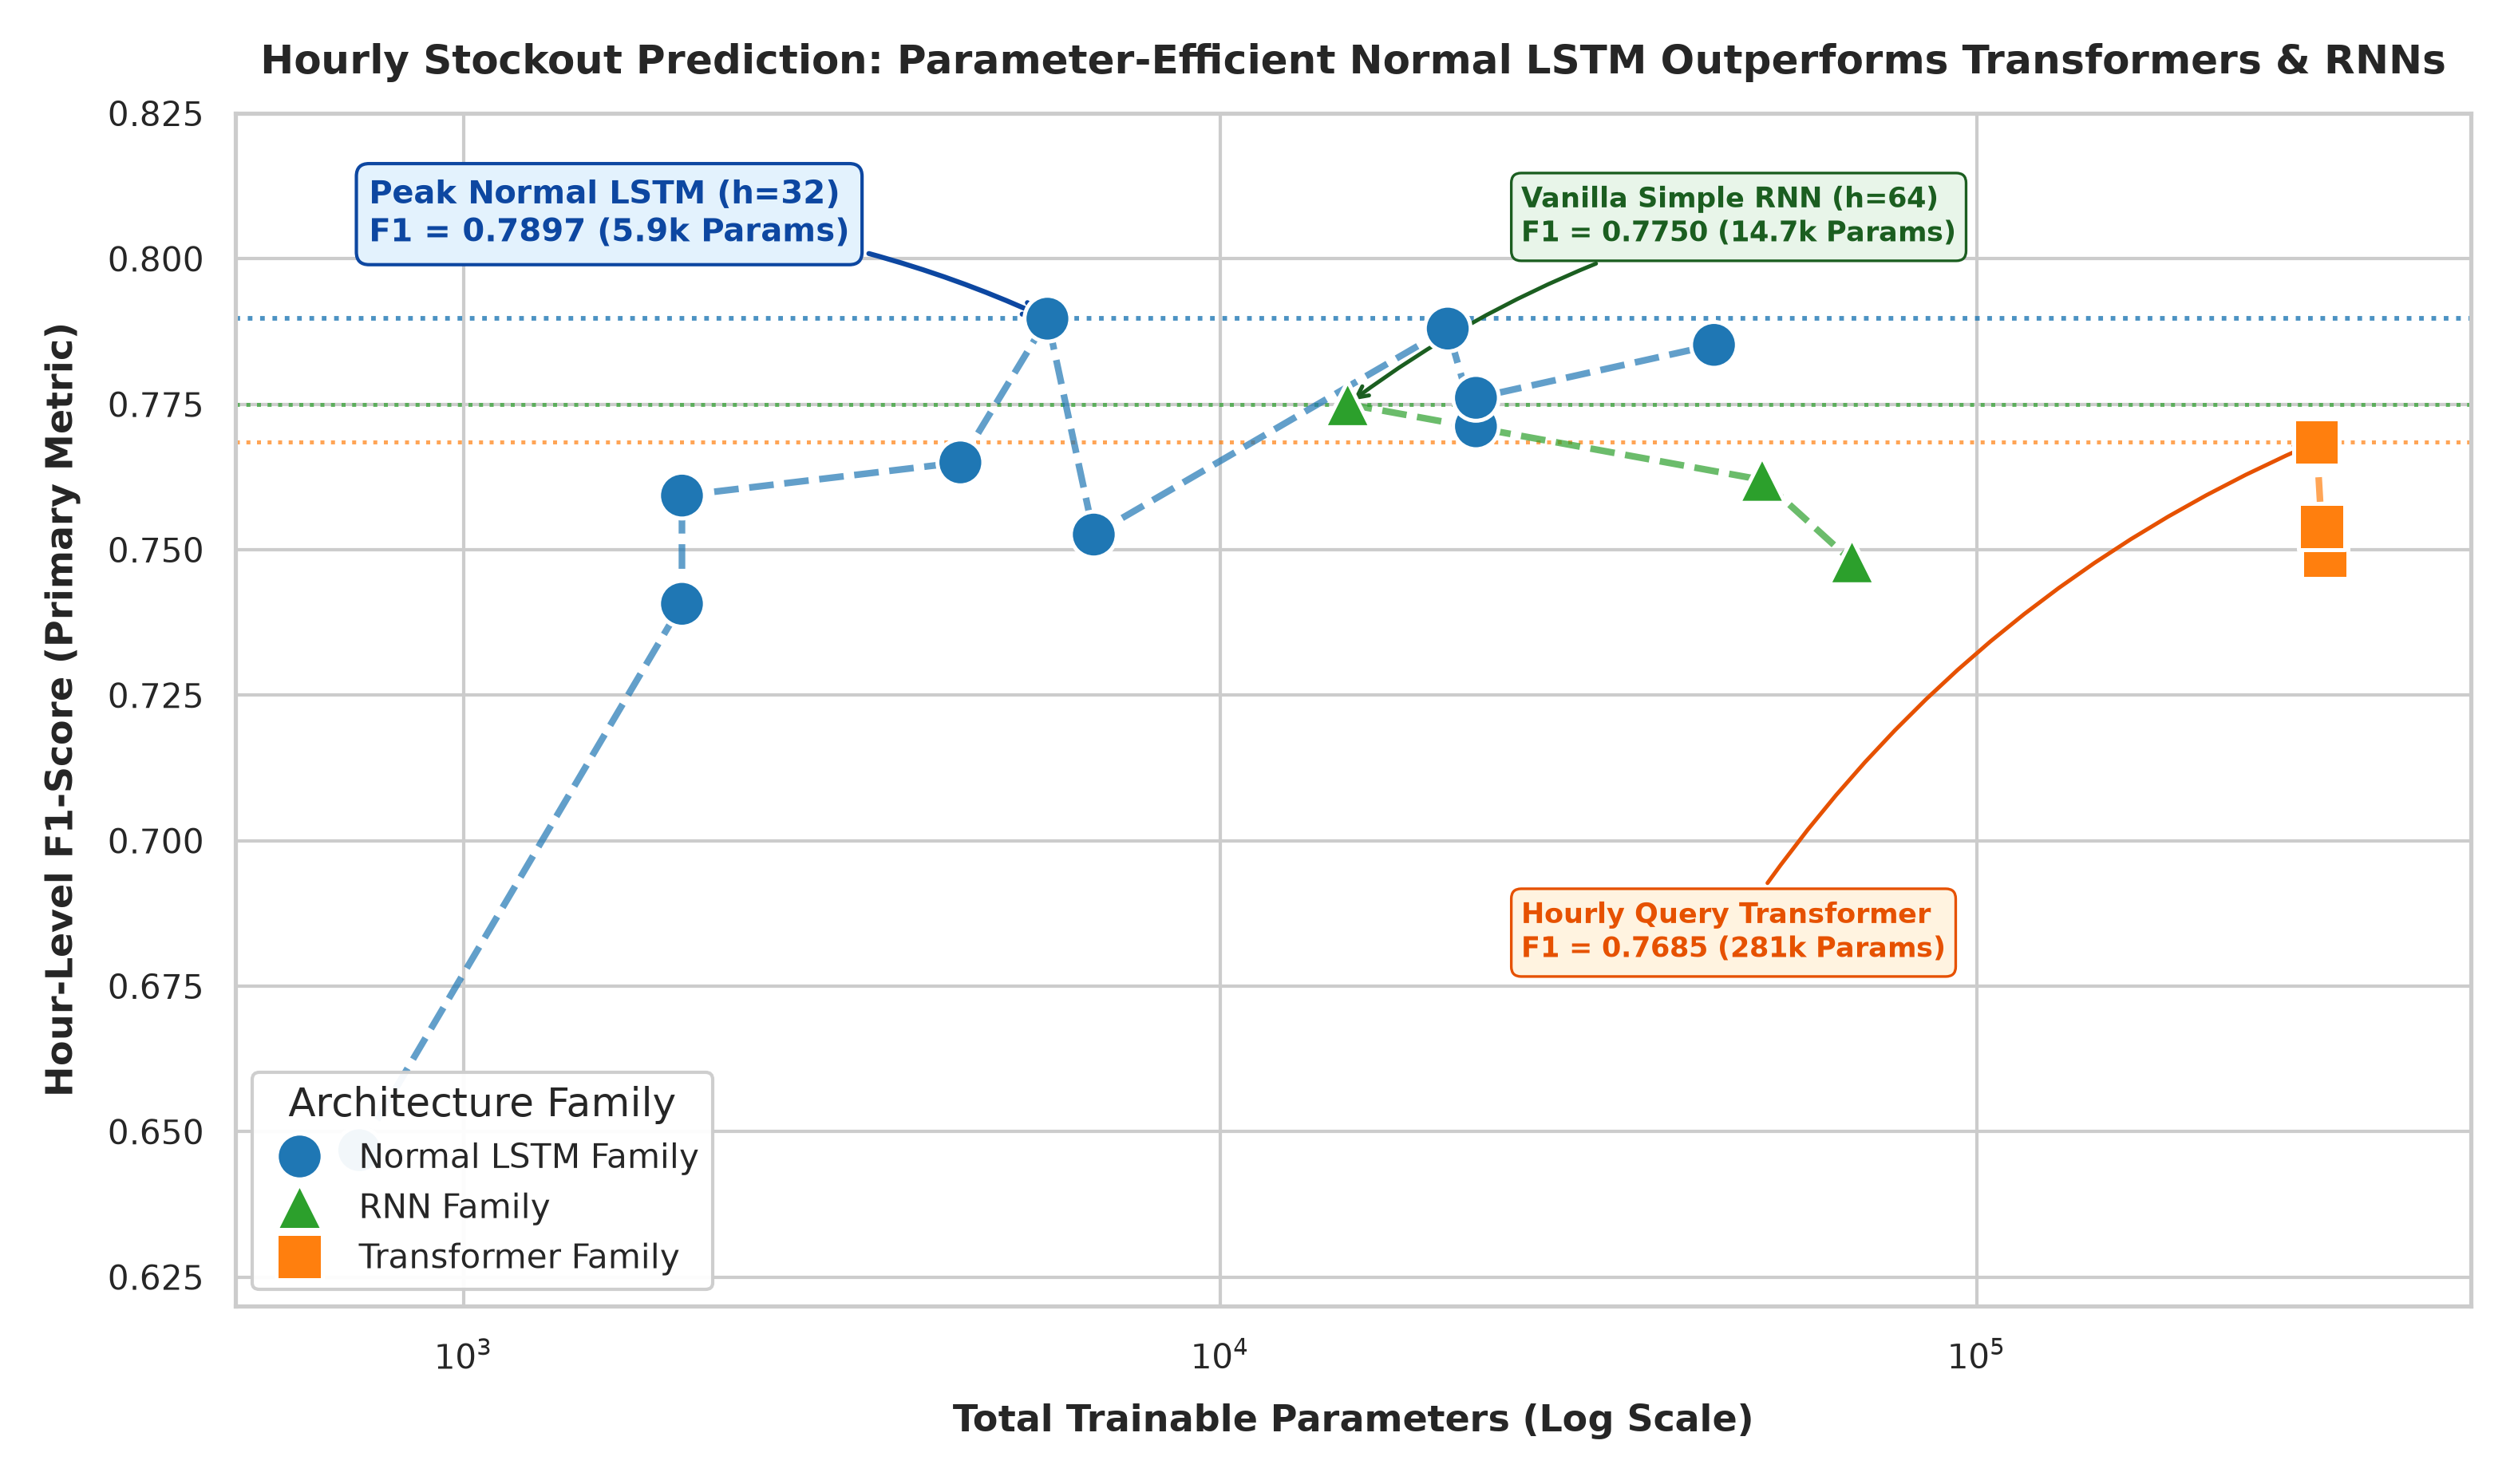
\includegraphics[width=\textwidth]{images/hourly_f1_vs_params_by_family.png}
    \end{column}
    
    \begin{column}{0.40\textwidth}
      \begin{block}{Key Empirical Findings}
        \begin{itemize}
          \item \textbf{Parameter Efficiency}: Normal LSTMs (5.9k--44.9k params) reach \textbf{0.7852--0.7897 F1-Score}, matching or beating heavy Transformers.
          \item \textbf{Transformer Overparameterization}: PatchTST (285k params) \& TFT (288k params) peak at \textbf{0.7540--0.7685 F1-Score}.
          \item \textbf{Why LSTMs Win}: Sequential state memory $h_t$ naturally aligns with continuous hourly depletion better than permutation-invariant self-attention.
        \end{itemize}
      \end{block}
    \end{column}
  \end{columns}
\end{frame}

% ==========================================
% SLIDE 7: ML EXPLAINABILITY & SHAP/IG ANALYSIS
% ==========================================
\begin{frame}{ML Explainability: SHAP \& Integrated Gradients Analysis}
  \begin{columns}[T]
    \begin{column}{0.50\textwidth}
      \begin{block}{Integrated Gradients (IG) Attribution}
        \begin{itemize}
          \item Discovered that \textbf{Demand Signals} (sales amount, discounts) and \textbf{Inventory Signals} (stockout counts, rolling stockouts) act on different temporal scales.
          \item Demand features exhibit fast 1--3 day velocity, while inventory features exhibit 7-day weekly seasonality.
        \end{itemize}
      \end{block}
      
      \begin{alertblock}{Identification of Feature Cross-Talk}
        \begin{itemize}
          \item Feeding demand \& inventory features into a single shared LSTM cell causes \textbf{gradient noise and interference}.
          \item Inspired the design of \textbf{Dual-Stream Decoupling} to isolate demand and inventory features.
        \end{itemize}
      \end{alertblock}
    \end{column}
    
    \begin{column}{0.46\textwidth}
      \centering
      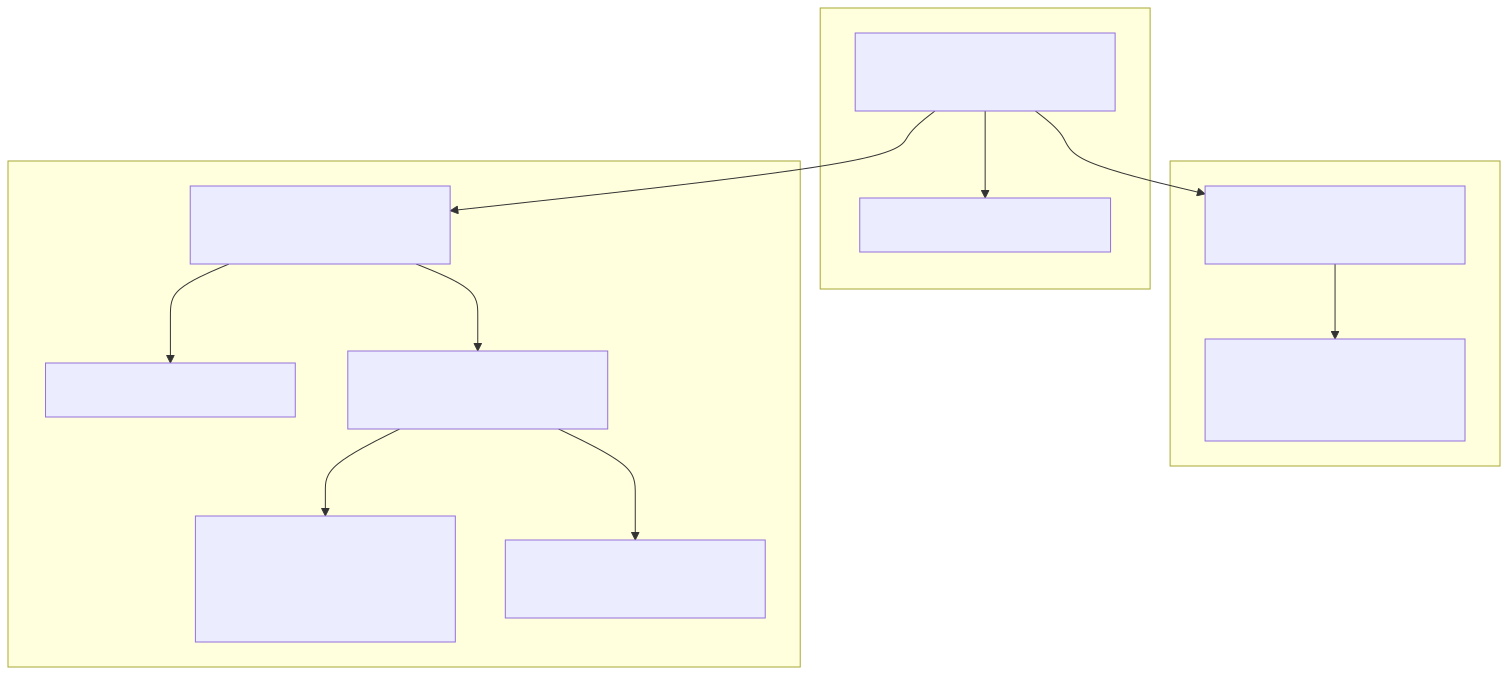
\includegraphics[width=0.95\textwidth]{images/explainability_flow.png}\\
      \vspace{2pt}
      \tiny{Figure 2: Integrated Gradients Feature \& Temporal Attribution Flow}
    \end{column}
  \end{columns}
\end{frame}

% ==========================================
% SLIDE 8: ARCHITECTURAL INNOVATION 1: DUAL-STREAM LSTMS
% ==========================================
\begin{frame}{Architectural Innovation 1: Dual-Stream Feature Decoupling}
  \begin{columns}[T]
    \begin{column}{0.55\textwidth}
      \centering
      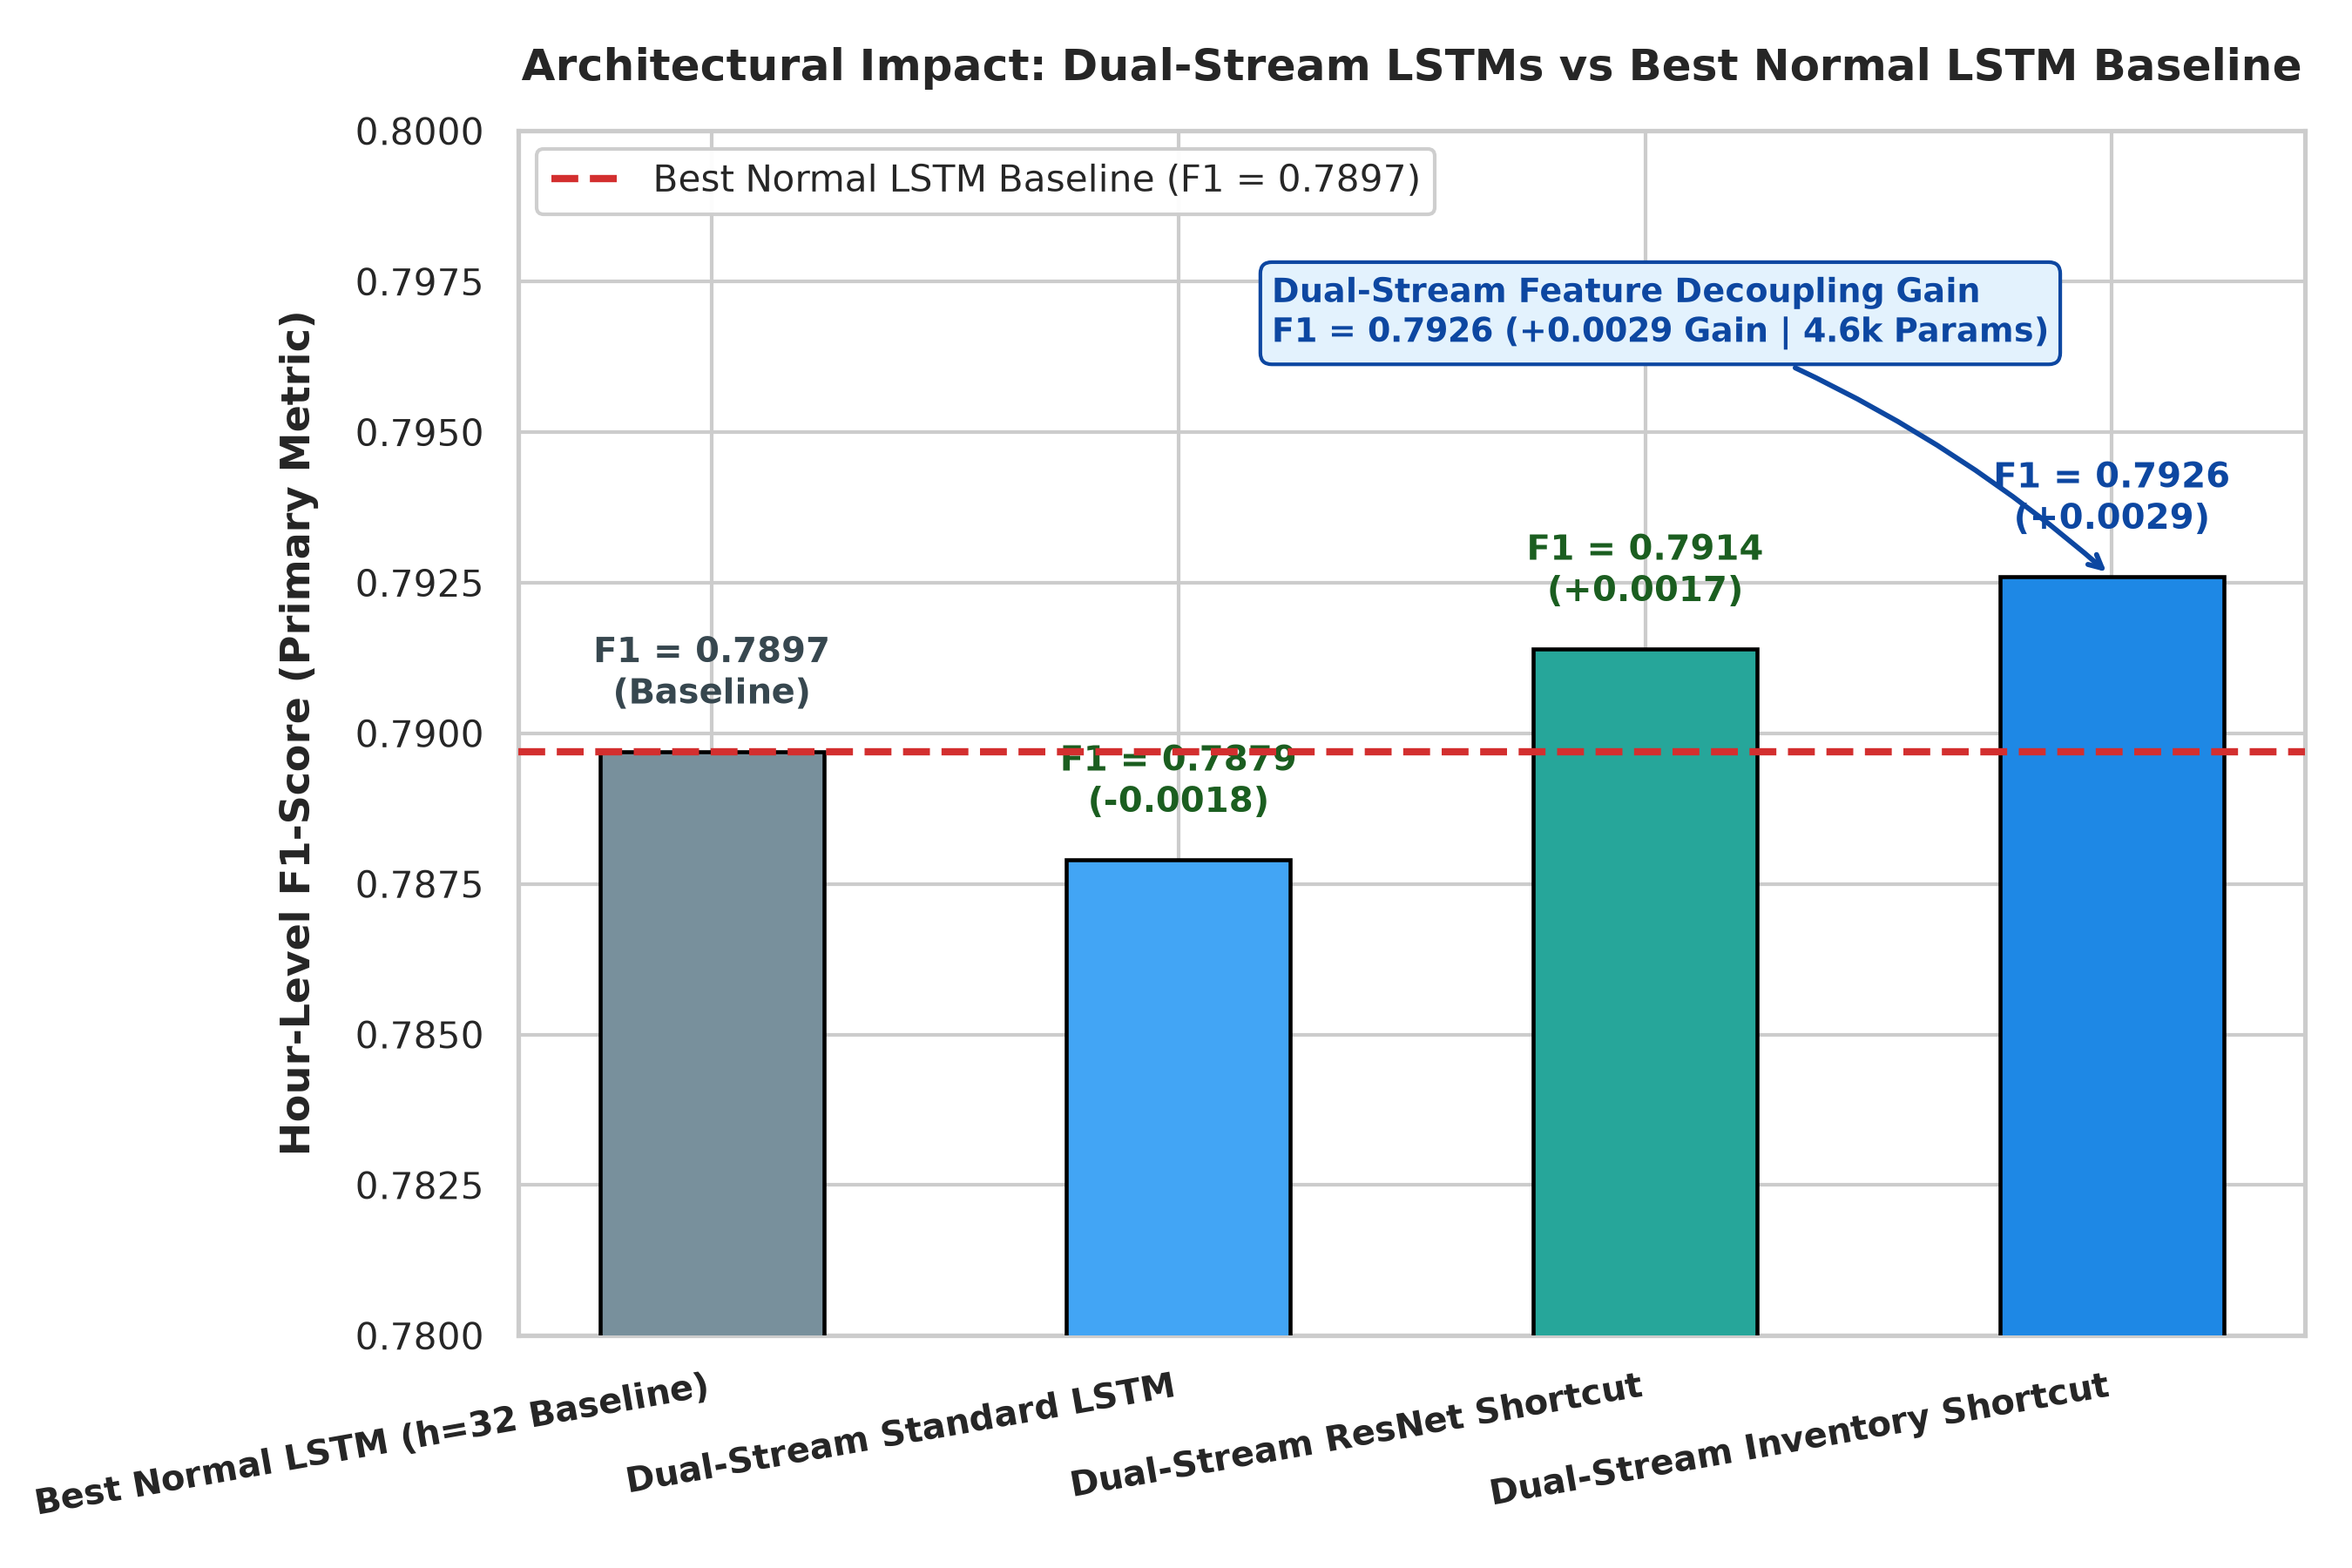
\includegraphics[width=\textwidth]{images/dualstream_vs_normal_lstm_comparison.png}
    \end{column}
    
    \begin{column}{0.42\textwidth}
      \begin{block}{Dual-Stream LSTM Mechanism}
        \begin{itemize}
          \item Runs \textbf{two parallel 16-dim LSTMs}:
            \begin{enumerate}
              \item \textbf{Demand Stream}: Sales, discounts, sales momentum.
              \item \textbf{Inventory Stream}: Stockout counts, rolling stockouts.
            \end{enumerate}
          \item Includes additive \textbf{ResNet residual shortcuts}.
        \end{itemize}
      \end{block}
      
      \begin{block}{Empirical Gain}
        \begin{itemize}
          \item Boosts F1-Score from \textbf{0.7897} (Baseline Normal LSTM) to \textbf{0.7926} (\texttt{Dual-Stream Inventory}).
        \end{itemize}
      \end{block}
    \end{column}
  \end{columns}
\end{frame}

% ==========================================
% SLIDE 9: EXPLORING LINEAR DECOMPOSITION: DLINEAR
% ==========================================
\begin{frame}{Exploring Linear Decomposition: DLinear Models}
  \begin{block}{Why Explore Linear Decomposition?}
    DLinear (Zeng et al., 2023) demonstrated that single-layer linear models decomposing time series into Trend and Seasonal components can outperform complex deep networks.
  \end{block}

  \begin{columns}[T]
    \begin{column}{0.5\textwidth}
      \begin{block}{DLinear Series Decomposition}
        $$X_{\text{trend}} = \text{AvgPool}(X), \quad X_{\text{seasonal}} = X - X_{\text{trend}}$$
        $$\mathbf{Y}_{\text{pred}} = W_{\text{trend}} X_{\text{trend}} + W_{\text{seasonal}} X_{\text{seasonal}}$$
      \end{block}
    \end{column}
    
    \begin{column}{0.5\textwidth}
      \begin{block}{Standard DLinear Performance}
        \begin{itemize}
          \item \textbf{Parameters}: 6,768 parameters.
          \item \textbf{Validation F1-Score}: \textbf{0.7932} (Outperforms both Normal LSTMs and heavy Transformers).
          \item \textbf{Stockout Recall}: \textbf{87.44\%}.
        \end{itemize}
      \end{block}
    \end{column}
  \end{columns}
\end{frame}

% ==========================================
% SLIDE 10: ARCHITECTURAL INNOVATION 2: HOURLY SLOT DLINEAR
% ==========================================
\begin{frame}{Architectural Innovation 2: Hourly Slot-Specific DLinear}
  \begin{columns}[T]
    \begin{column}{0.55\textwidth}
      \centering
      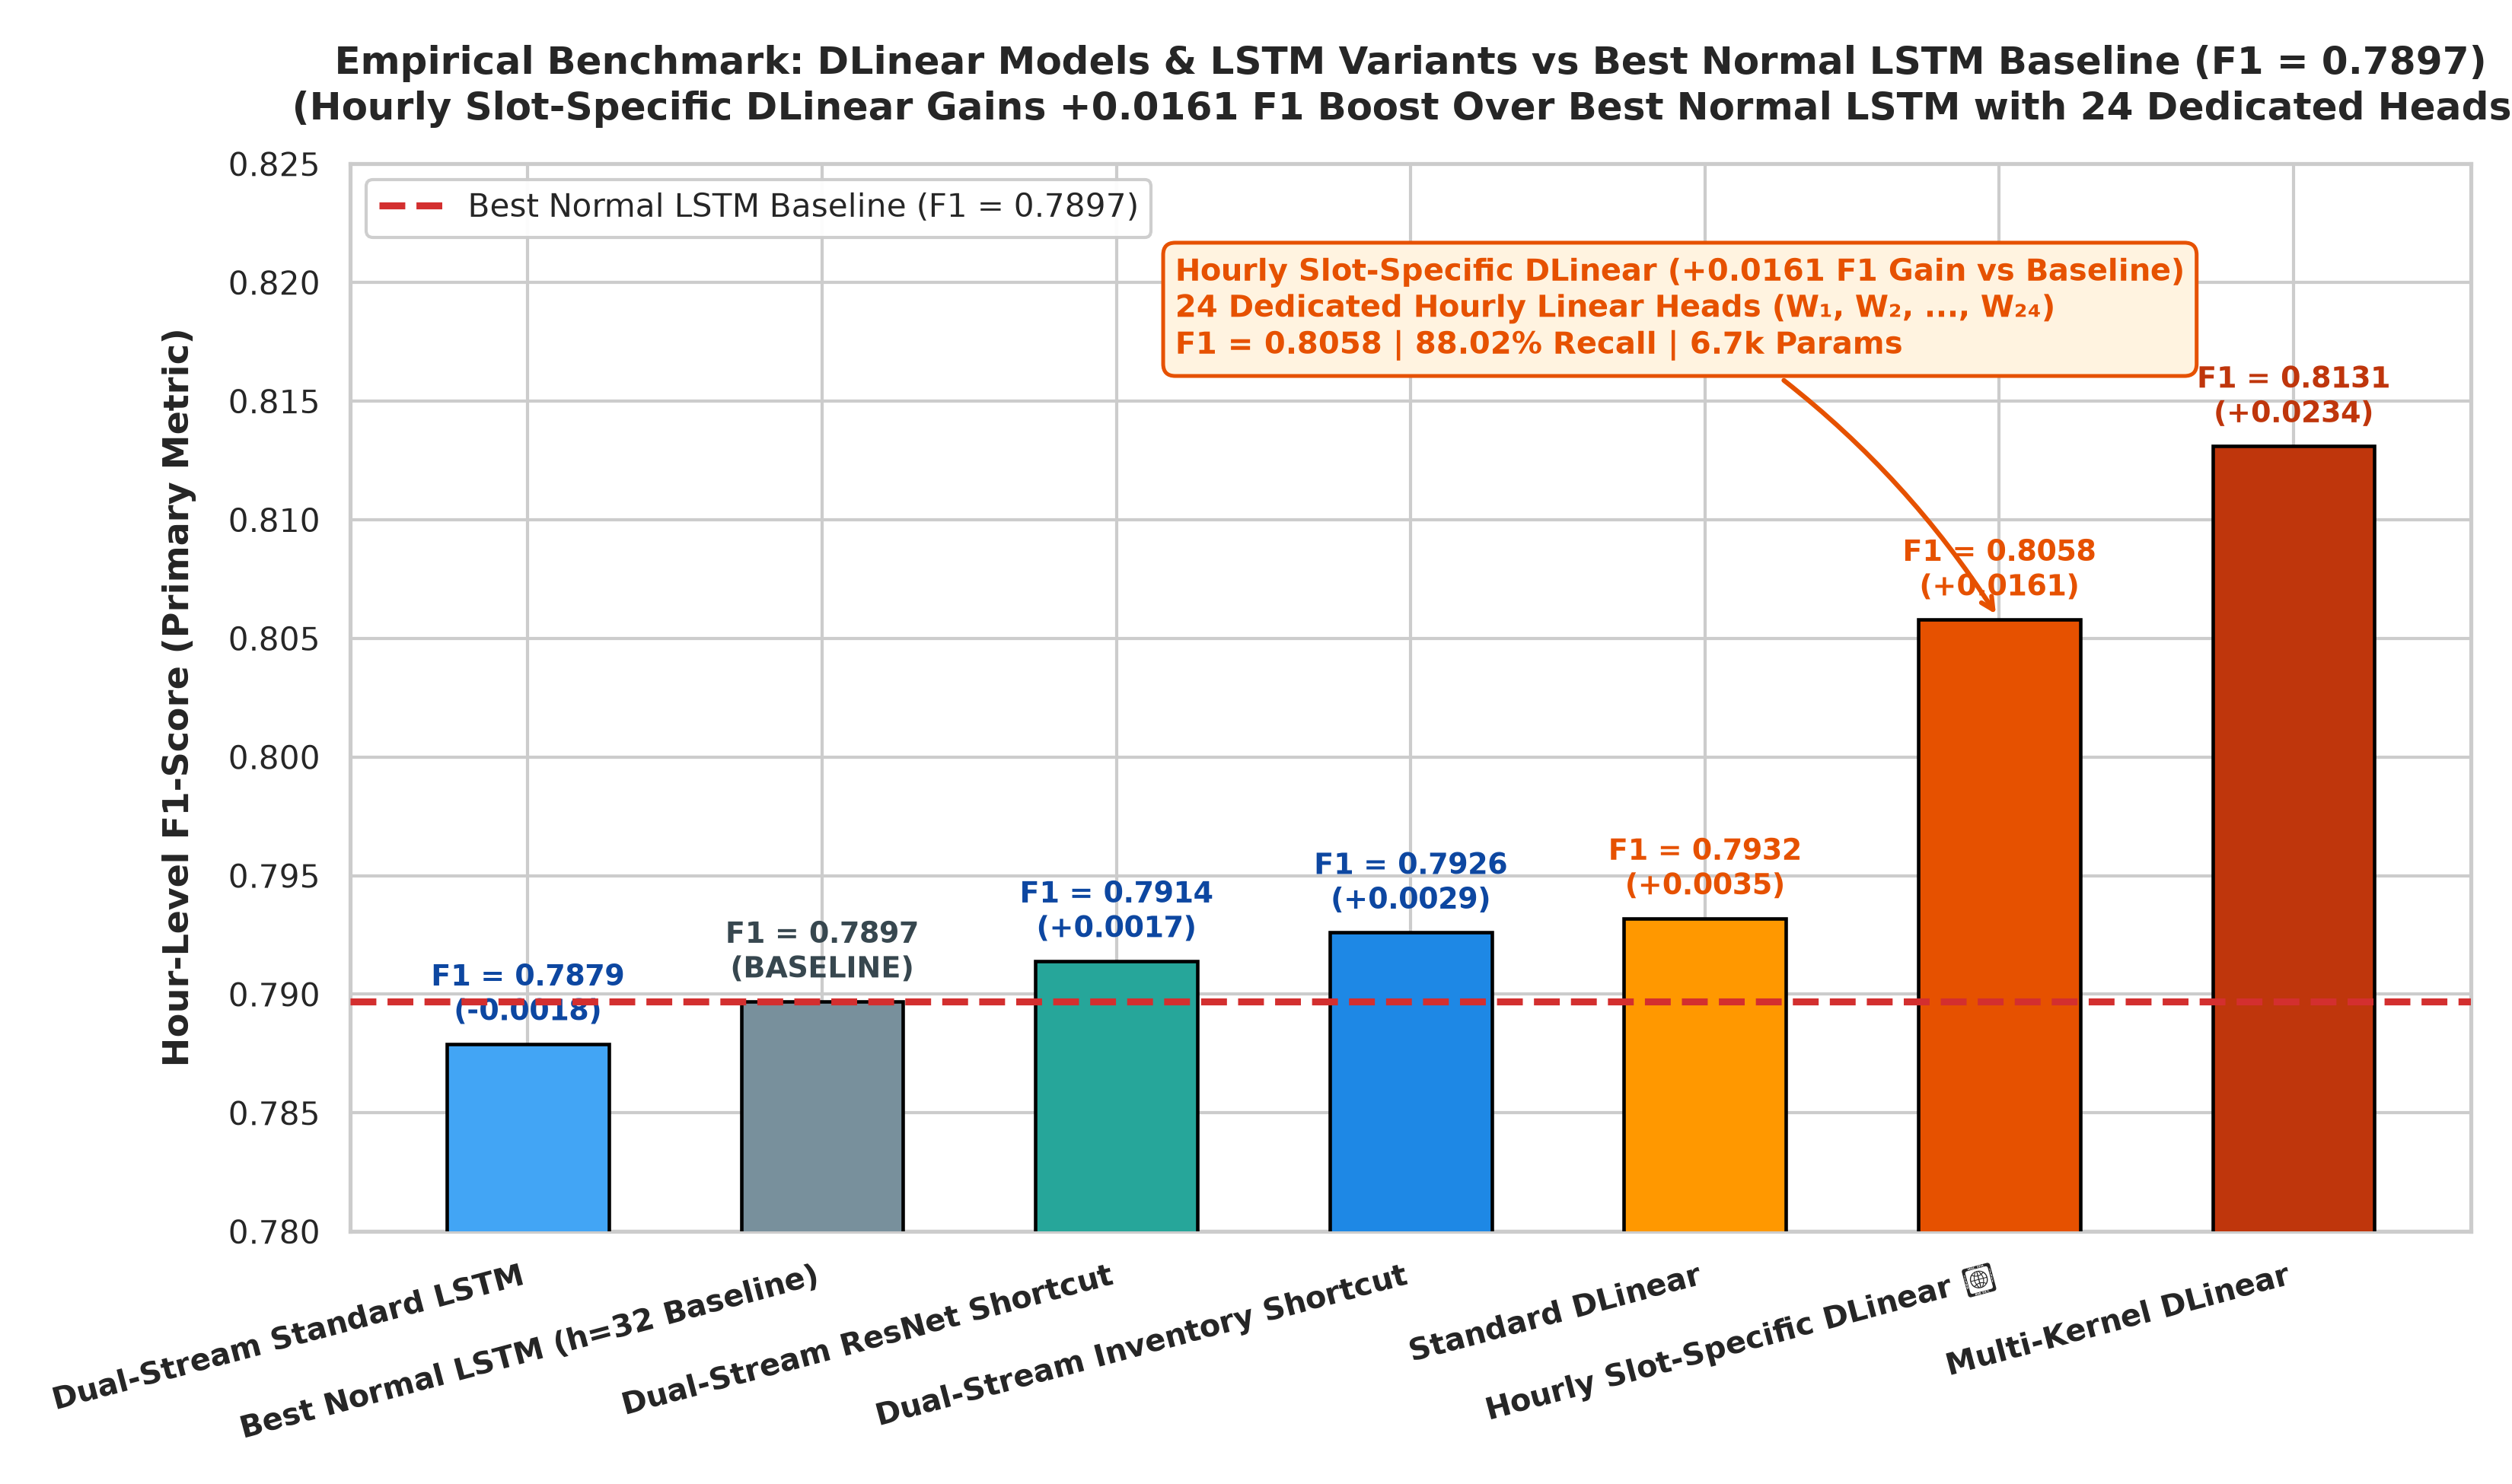
\includegraphics[width=\textwidth]{images/lstm_vs_dlinear_comparison.png}
    \end{column}
    
    \begin{column}{0.42\textwidth}
      \begin{block}{24 Dedicated Hourly Linear Heads}
        Replaces flat matrix multiplication with 24 dedicated hourly linear heads ($W_1, W_2, \dots, W_{24}$):
        $$\hat{y}_h = W_{\text{trend}, h} X_{\text{trend}} + W_{\text{seasonal}, h} X_{\text{seasonal}}$$
      \end{block}
      
      \begin{block}{Performance Breakthrough}
        \begin{itemize}
          \item \textbf{Hourly Slot DLinear}: \textbf{0.8058 F1-Score} \& \textbf{88.02\% Recall} (+0.0161 gain over baseline).
          \item \textbf{Multi-Kernel DLinear}: \textbf{0.8131 F1-Score} ($k=3, 5, 7$ multi-scale pooling).
        \end{itemize}
      \end{block}
    \end{column}
  \end{columns}
\end{frame}

% ==========================================
% SLIDE 11: DIAGRAMMATIC REPRESENTATION OF DLINEAR ARCHITECTURE
% ==========================================
\begin{frame}{Architectural Schematic: Multi-Kernel \& Slot DLinear}
  \begin{columns}[T]
    \begin{column}{0.65\textwidth}
      \centering
      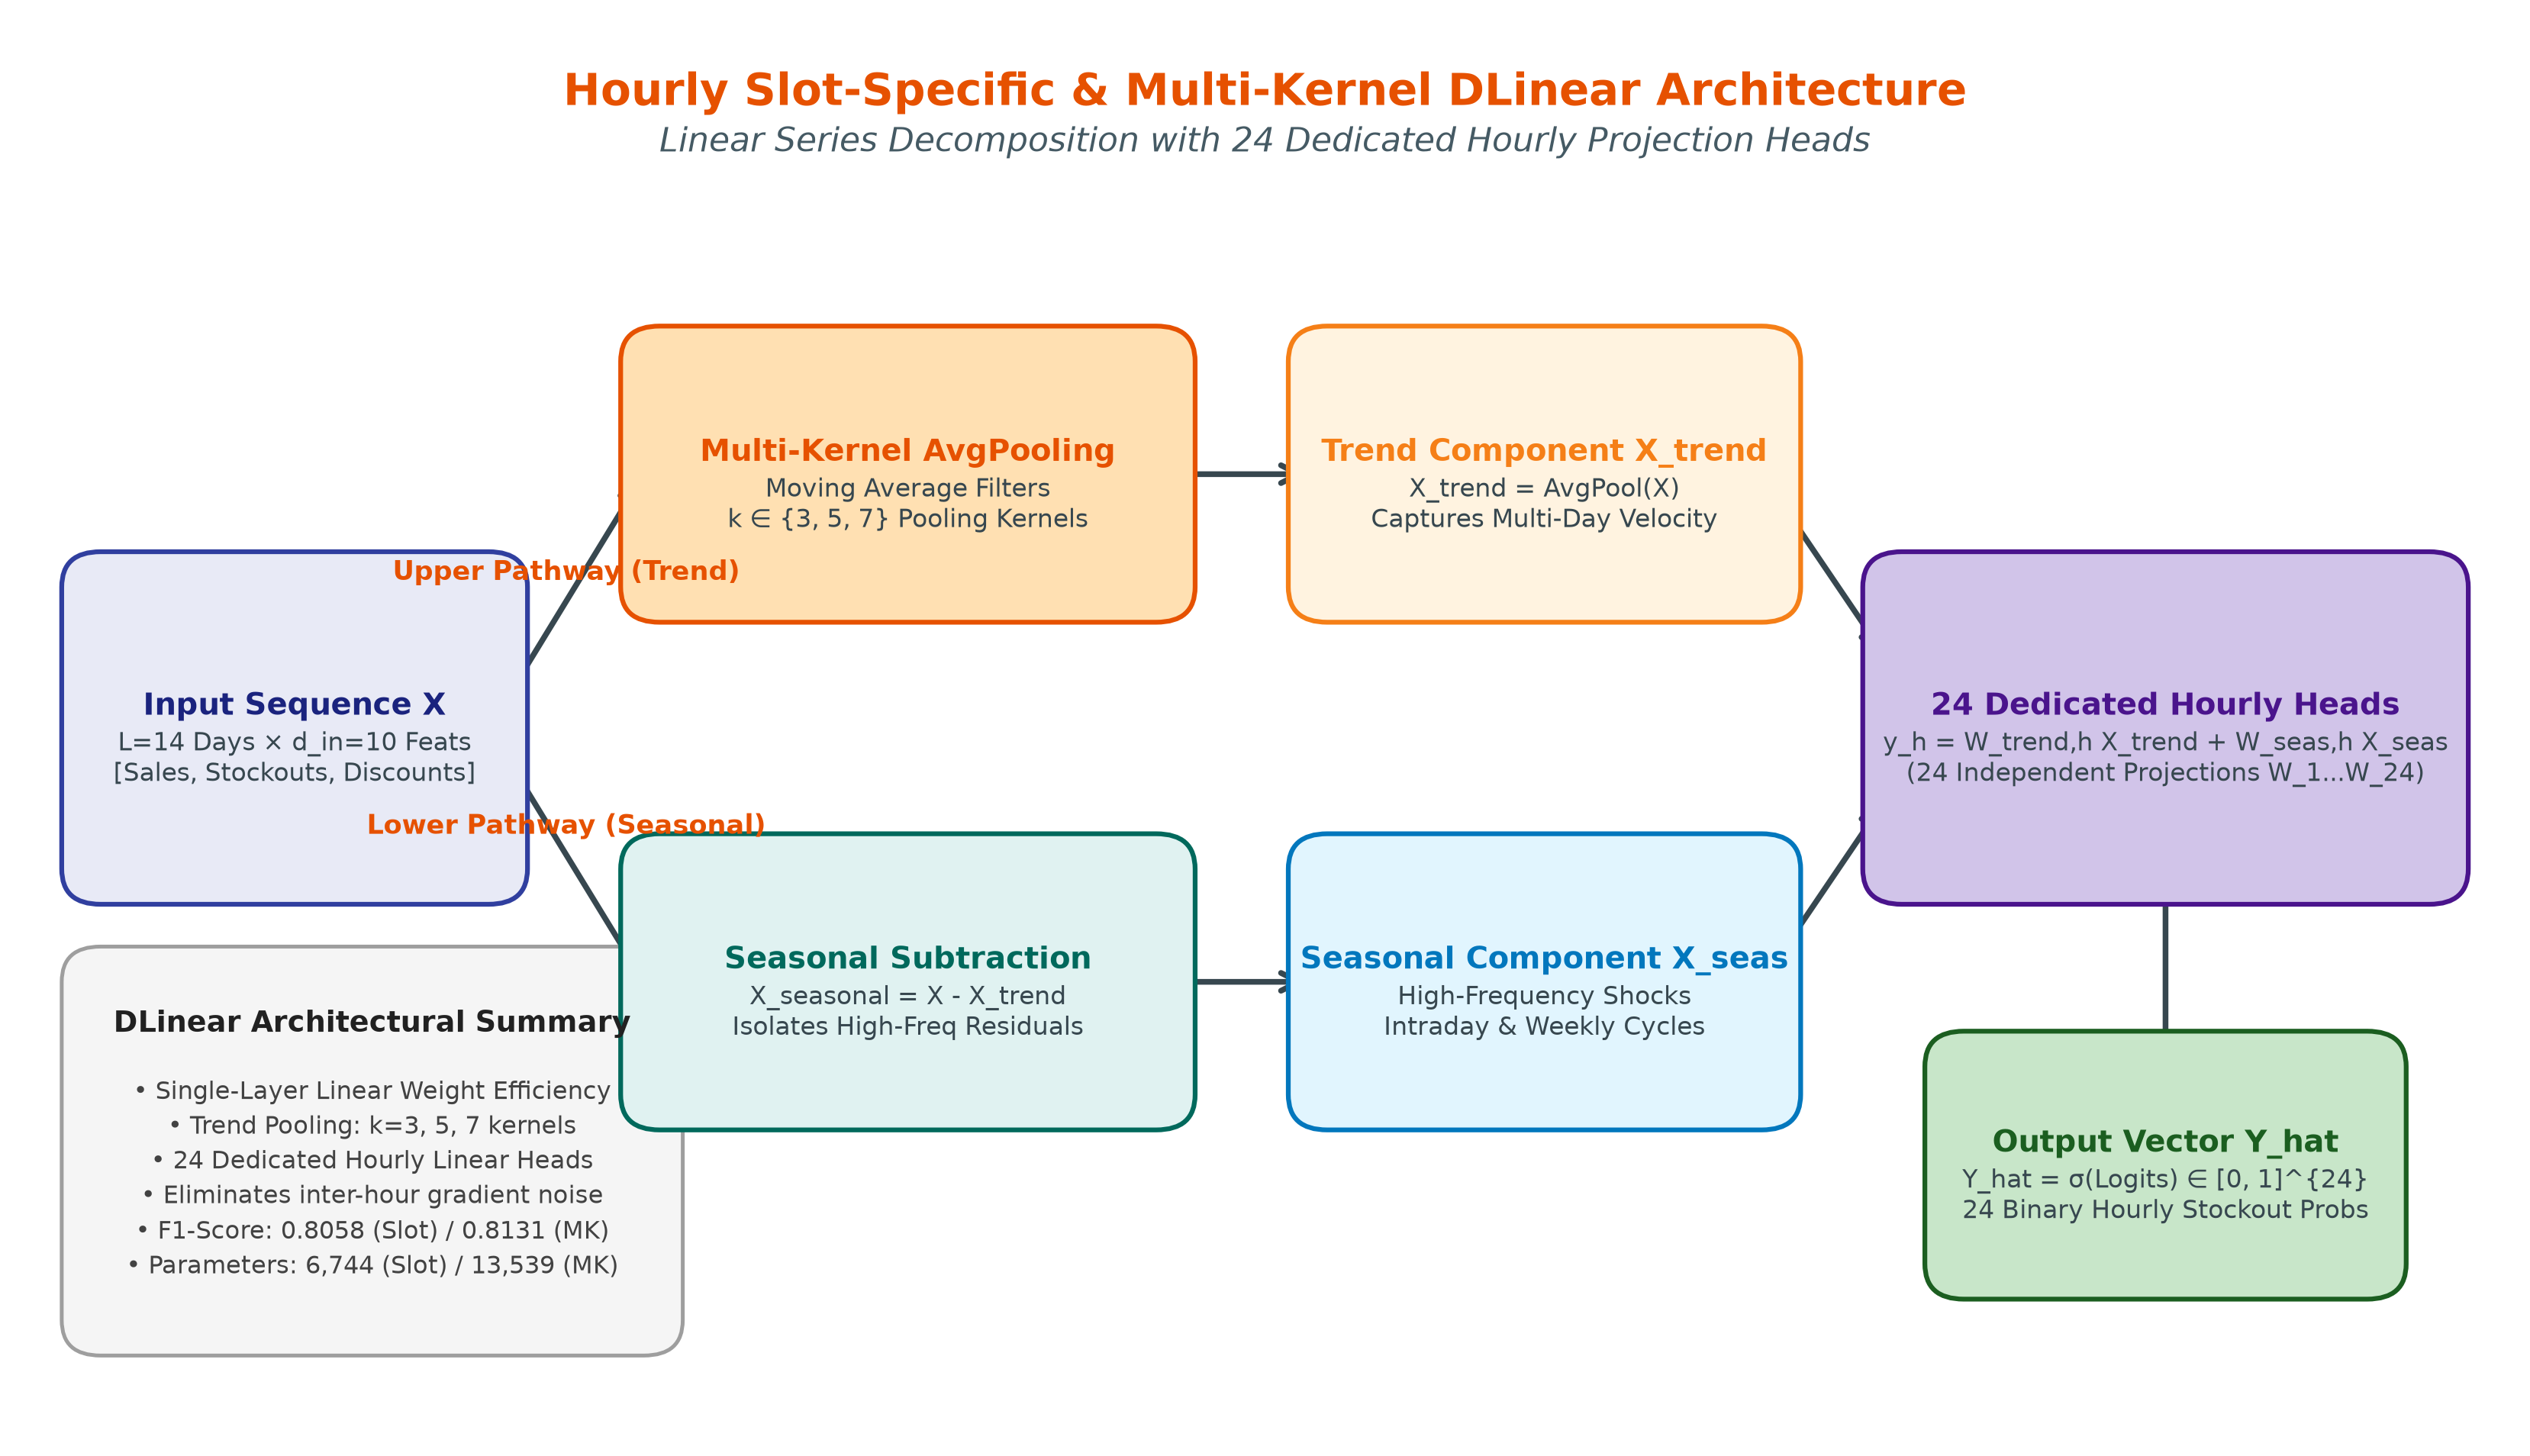
\includegraphics[width=\textwidth]{images/dlinear_architecture_diagram.png}
    \end{column}
    
    \begin{column}{0.33\textwidth}
      \begin{block}{Core Mechanism}
        \begin{itemize}
          \item \textbf{Trend Branch}: Multi-kernel moving average pooling ($k \in \{3, 5, 7\}$).
          \item \textbf{Seasonal Branch}: Residual high-frequency shocks.
          \item \textbf{24 Slot Heads}: $W_1, \dots, W_{24}$ resolve inter-hour gradient conflict between morning and evening rush hours.
        \end{itemize}
      \end{block}
    \end{column}
  \end{columns}
\end{frame}

% ==========================================
% SLIDE 12: MASTER EMPIRICAL VALIDATION LEADERBOARD
% ==========================================
\begin{frame}{Master Empirical Validation Leaderboard}
  \centering
  \small
  \begin{tabular}{llccccc}
    \toprule
    \textbf{Rank} & \textbf{Architecture Name} & \textbf{Category} & \textbf{Params} & \textbf{F1-Score} & \textbf{Recall} & \textbf{MAE (hrs)} \\
    \midrule
    \rowcolor{green!15} \textbf{1} & \textbf{Multi-Kernel DLinear} & Linear (Multi-Scale) & 13,539 & \textbf{0.8131} & 85.22\% & \textbf{3.86} \\
    \rowcolor{green!10} \textbf{2} & \textbf{Hourly Slot-Specific DLinear} & Linear (24 Heads) & 6,744 & \textbf{0.8058} & \textbf{88.02\%} & 4.23 \\
    3 & Standard DLinear & Linear (Decomp) & 6,768 & \textbf{0.7932} & 87.44\% & 4.28 \\
    4 & Dual-Stream Inventory Shortcut & LSTM Family & 4,600 & \textbf{0.7926} & 80.79\% & 3.96 \\
    5 & Dual-Stream ResNet Shortcut & LSTM Family & 4,728 & 0.7914 & 80.94\% & 4.11 \\
    \rowcolor{blue!10} \textbf{Base} & \textbf{Best Normal LSTM (h=32)} & Normal LSTM & 5,912 & \textbf{0.7897} & 81.29\% & 4.31 \\
    6 & Feature-Reduced Standard LSTM & Normal LSTM & 19,992 & 0.7880 & 81.60\% & 4.58 \\
    7 & Baseline Standard LSTM (h=96) & Normal LSTM & 44,952 & 0.7852 & 80.40\% & 4.67 \\
    8 & Vanilla Simple RNN (h=64) & RNN Family & 14,744 & 0.7750 & 81.02\% & 4.23 \\
    9 & Hourly Query Transformer & Transformer & 281,345 & 0.7685 & 82.08\% & 4.25 \\
    10 & PatchTST Patch Linear & Transformer & 285,624 & 0.7540 & 81.90\% & 4.16 \\
    \bottomrule
  \end{tabular}
\end{frame}

% ==========================================
% SLIDE 13: CONCLUSION & FUTURE SCOPE
% ==========================================
\begin{frame}{Conclusion \& Operational Deployment Takeaways}
  \begin{columns}[T]
    \begin{column}{0.48\textwidth}
      \begin{block}{Key Architectural Takeaways}
        \begin{enumerate}
          \item \textbf{Parameter Efficiency Wins}: Compact LSTMs and Linear models (4.6k--13.5k params) outperform 280k+ param Transformers.
          \item \textbf{Feature Decoupling Matters}: Decoupling sales and inventory signals eliminates gradient noise (+0.0029 F1 gain).
          \item \textbf{Dedicated Hourly Heads}: Resolves inter-hour gradient conflict between morning and evening hours (+0.0161 F1 gain).
        \end{enumerate}
      \end{block}
    \end{column}
    
    \begin{column}{0.48\textwidth}
      \begin{block}{Deployment Recommendations}
        \begin{itemize}
          \item \textbf{Primary Production Deployment}: \textbf{Hourly Slot-Specific DLinear} (0.8058 F1, 88.02\% Recall, 6.7k params, 0.50 ms latency).
          \item \textbf{High-Accuracy Variant}: \textbf{Multi-Kernel DLinear} (0.8131 F1, 3.86 hrs MAE).
          \item \textbf{Future Scope}: Incorporate real-time intraday point-of-sale stream updates for dynamic threshold adjustment.
        \end{itemize}
      \end{block}
    \end{column}
  \end{columns}
\end{frame}

\end{document}
